\chapter{Wave Motion}

The world is full of waves, with \textit{mechanical} and \textit{electromagnetic}
waves being the two main types. 
\begin{itemize}
    \item \textbf{Mechanical waves} requires that some physical medium being disturbed.
        For example, the water in a pond is disturbed when you throw a rock into it.
    \item \textbf{Electromagnetic waves} does not require a medium. For example, light can
        travel through empty space without a medium. For now, we will focus on mechanical waves.
\end{itemize}

For now, we will only focus on mechanical waves. Consider again the rock being dropped onto water.
The disturbed water molecules gains kinetic energy from the rock, and it can be transfer to another
object floating on water, causing it to move. Notice that the energy is transferred over distance,
but not matter. Also notice that the molecules of the disturbed water resembles periodic motion of
a vibrating pendulum.

\section{Propogation of a Disturbance}

All mechanical waves require the following
\begin{enumerate}
    \item a source of disturbance
    \item a medium with elements that can be disturbed
    \item a physical mechanism that allows each element to influence each other
\end{enumerate}

A \textbf{pulse} is a single wave of disturbance being transferred through a medium where each element 
of the medium is disturbed. The pulse travels along the medium with definite speed.
Consider the following example
\begin{center}
    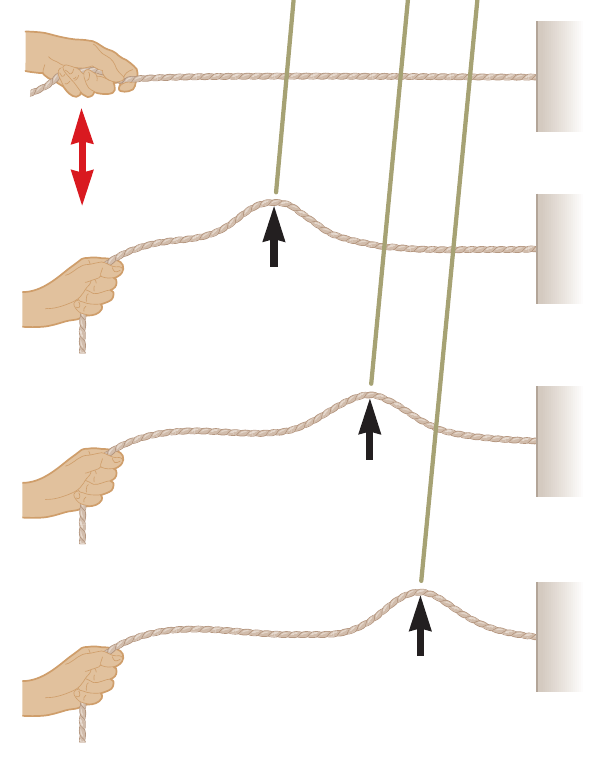
\includegraphics[scale=0.3]{images/oaw/pod01.png}
\end{center}

In this example, the hand is the source of the disturbance, the string is the medium, and the fact 
that the string is connected allows the pulse to travel through the string, disturbing each element 
of the string in the process. Also notice that the pulse has a certain height and speed and the 
shape of the pulse changes very little throughout the whole motion.

\subsection{Types of Disturbance}

Consider a pulse (or wave) traveling along the string. If the elements of the disturbed medium are
moving perpendicular to the direction of propogation, we call said wave a \textbf{transverse wave}.
The pulse on the string example from above is an example of a transverse wave.
In contrast, if the elements of the disturbed medium are moving parallel to the direction of propogation,
we call said wave a \textbf{longitudinal wave}. For example, creating a compressed region on a spring
that moves along it is an example of a longitudinal wave.
\begin{center}
    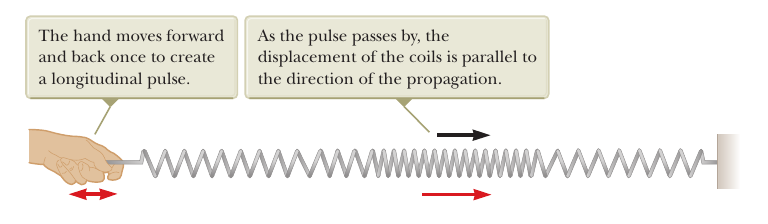
\includegraphics[scale=0.7]{images/oaw/pod02.png}
\end{center}

Some waves in nature are a combination of transverse and longitudinal waves. For example, surface 
water waves actually move in circular path, meaning the disturbance has both transverse and longitudinal
components to it.
\begin{center}
    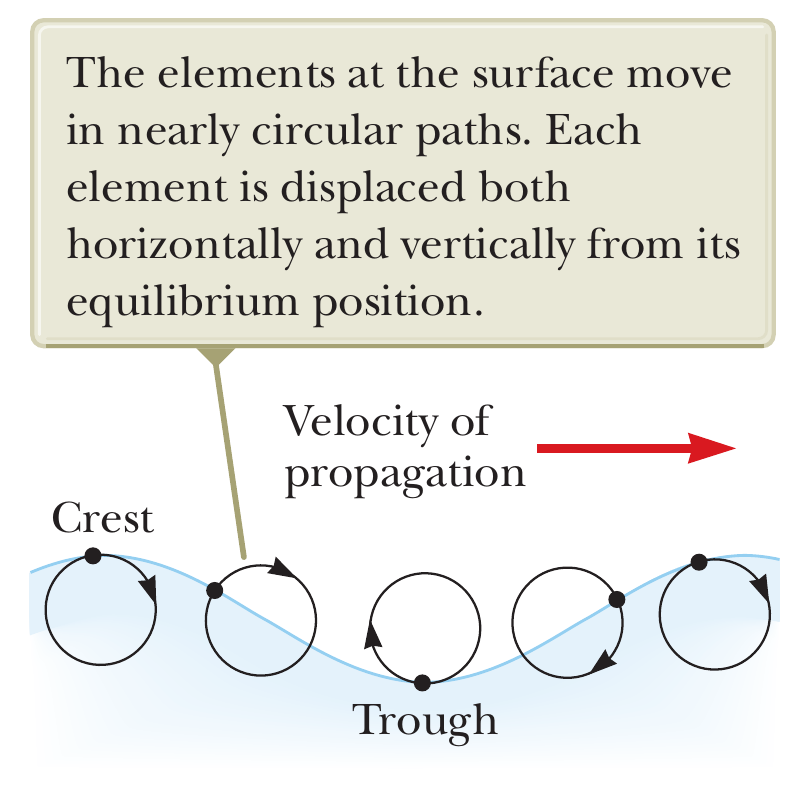
\includegraphics[scale=0.25]{images/oaw/pod03.png}
\end{center}

\subsection{Wave Function}